\section{Renewable Energy Demonstrator Testbench}
\label{REDtestbench}

\begin{figure}[htbp]
    \centering
    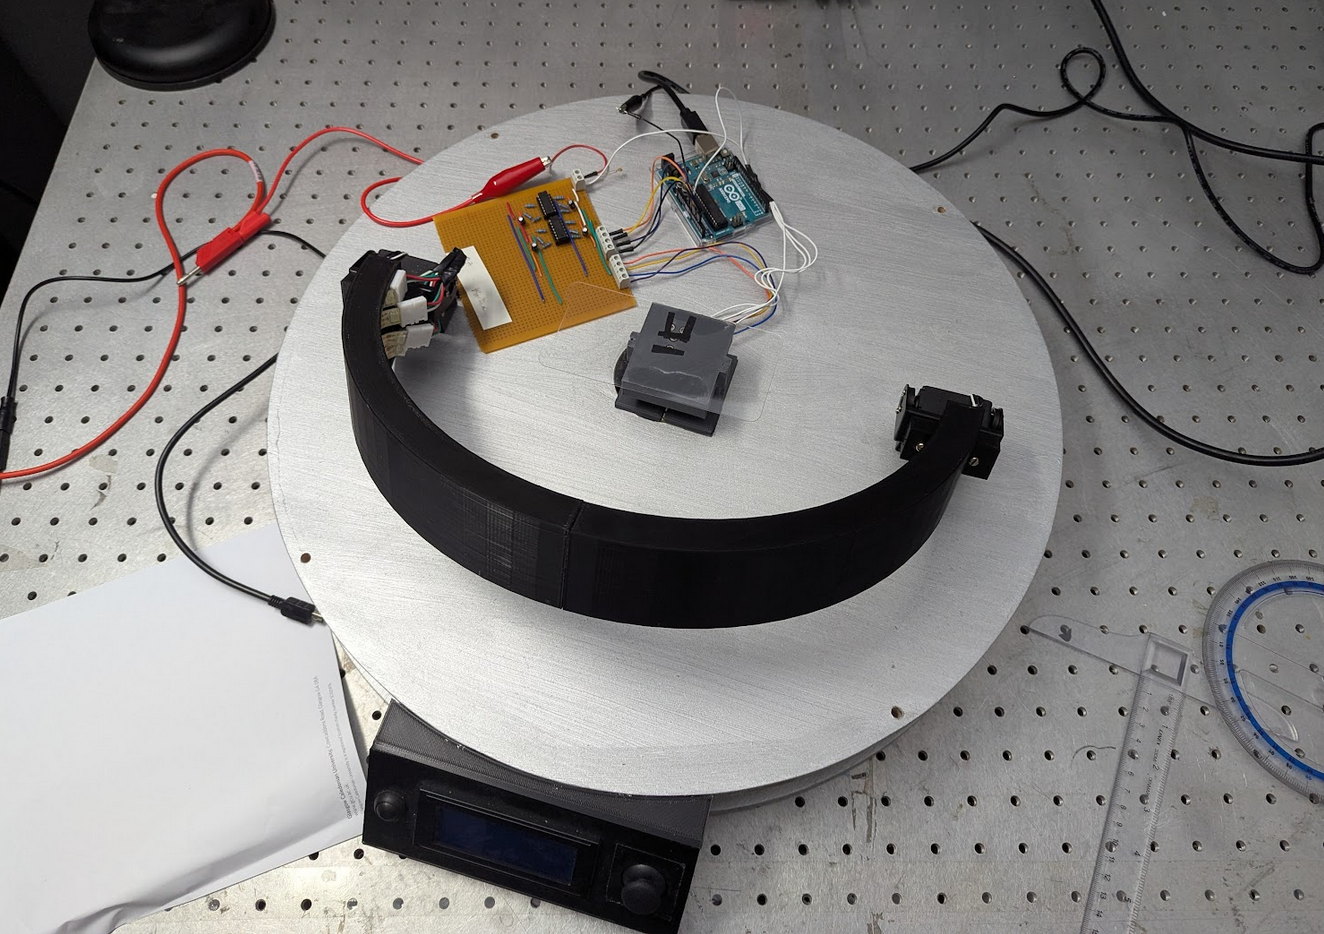
\includegraphics[width=0.7\textwidth]{chapters/methodology/RED/RED_image.png}
    \caption{The RED Testbench modified to fit our sensor} 
    \label{fig:RED_testbench_flowchart}
\end{figure}

For testing the capability of the Sun Sensor to correctly detect the location of the light source, a test bench was required that could reliably place the location of the light at a precise location repeatedly. For this purpose we used a project built by our colleagues in the \acf{EPS} year 2021/22 who created just such a device intended for demonstrating renewable energy creation live and interactive~\cite{RefWorks:shopov2022renewable}. Their device was able to demonstrate the energy levels created by a \ac{PV} cell by light emitted at different angles. The light emission would change location based on time of day and the PV cell readings would show the difference in energy. Further, the PV cell was controllable by a joystick to point the PV Cell at the optimum angle for the highest energy capture. For our project, the arch and LED strip were used for outputting light from different angles. The photovoltaic cell was removed together with the servomotor to make space for our \ac{PSD} device.  The \ac{RED} device was composed of two separate Arduino microcontrollers:
\begin{itemize}
    \item Arduino Uno - for controlling the Arch 
    \item Arduino Nano - for controlling the LED Strip
\end{itemize}

The \textbf{Arduino Uno} is the main controller which not only controlled the Arch assembly, but also acted as the primary controller, receiving inputs from a button and joystick, updating an LCD screen and sending an impulse to the secondary Arduino Nano for controlling the LED Strip. A photo of the \ac{RED} Testbench is available in Figure \ref{fig:RED_testbench_flowchart}.

The \textbf{Arduino Nano} is the secondary controller that receives a digital signal from the 

\subsection{LED Controller reprogramming}
Once the \ac{RED} was modified by removing the servo in the middle, both the LED controller and the  main controller had to be reprogrammed. This was an easy task as we had access to the original code and permission from the RED \cite{RefWorks:shopov2022renewable} team to modify it. For the LED controller, two versions were created:

One version that more closely resembles the original code, listens to the signal on a digital pin from the main arduino, and change to the next position out of a total of five positions.

A second version of the LED controller was created that simply changed which group of $3 \cdot 3$ LEDs were turned on every 5 seconds. This was required to perform a dynamic test where the datastream would be recorded to compare with simulation. The full code is available in Appendix \ref{app:AppendixF}. This version was a "hack" that allowed us to record a moving light with the arch set to stay at 90\textdegree() (one of the original 5 positions). 

The flowchart shows the basic operation is reproduced in Figure \ref{fig:REDarchflowchart}. The final design has the following angles:

  \begin{table}[htbp]
    \centering
    \caption{Arch and RGB LED Coordinates in Hemispherical System}
    \begin{tabular}{|c|c|c|c|}
    \hline
    \textbf{Preset} & \textbf{Altitude} & \textbf{Approximate} & \textbf{RGB LED} \\
    \textbf{Position} & \textbf{(degrees)} & \textbf{Azimuth (degrees)} & \textbf{Position} \\
    \hline
    1 & 20 & 20 & 3 \\
    \hline
    2 & 50 & 50 & 9 \\
    \hline
    3 & 90 & 90 & 13 \\
    \hline
    4 & 130 & 130 & 17 \\
    \hline
    5 & 160 & 160 & 23 \\
    \hline
    \end{tabular}
    \label{tab:arch-led-positions}
\end{table}


  
The angles chosen to record data were randomly selected, and for simplicity and ease of measurement (manually with protractor) the altitude and azimuth were identical. These were then reproduced in simulation as per Section \ref{sec:softwareModel}. The simplicity was also intended to avoid confusion between team members working on separate parts of the project.

\subsection{Arch Movement Reprogramming}
%%%%%%%%%%%%%%%%%
% ARCH Flowchart
\begin{figure}[htbp] 
  \centering
  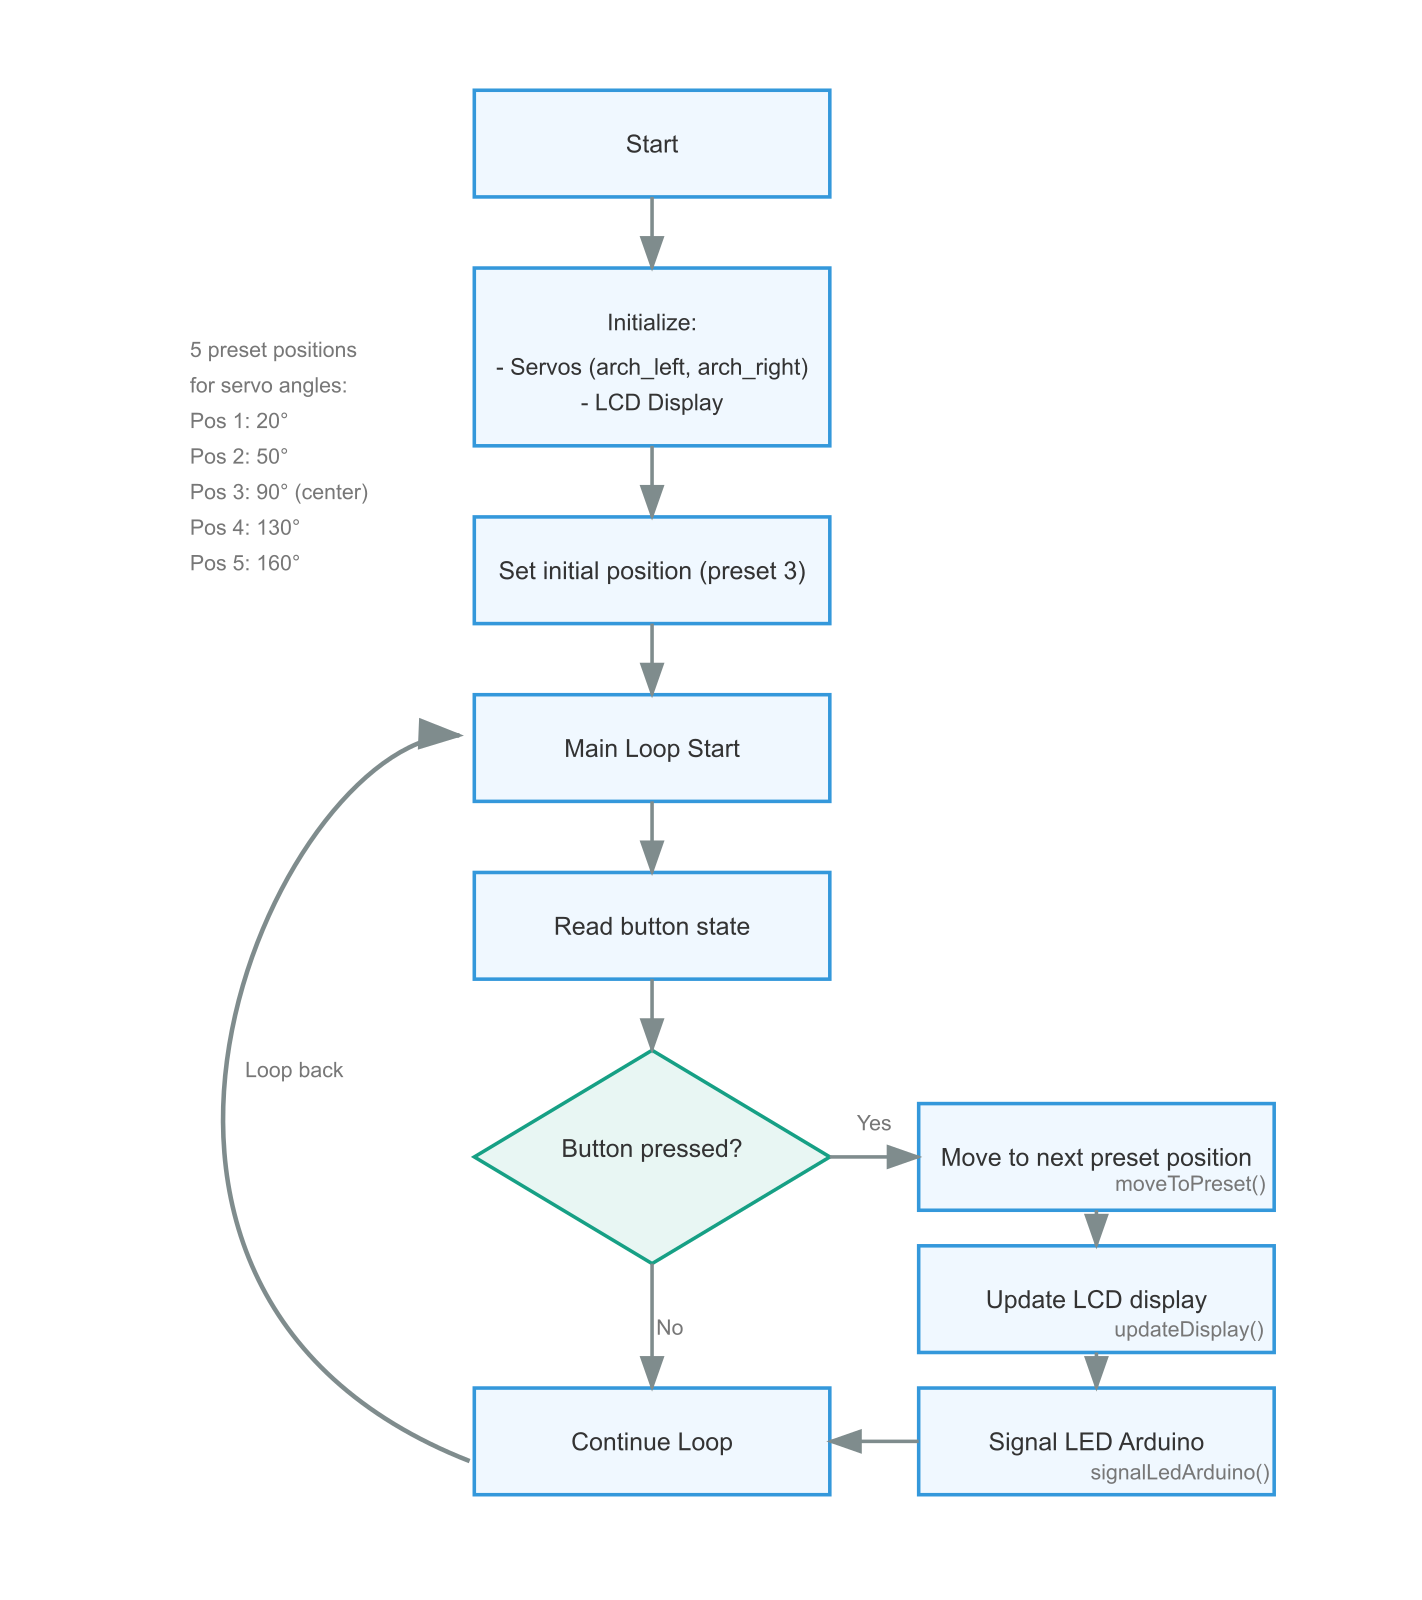
\includegraphics[width=0.95\textwidth]{chapters/methodology/RED/arch_flow.png}
  \caption{Flowchart of the C++ program on the Arduino Controlling the Arch and other peripherals}
  \label{fig:REDarchflowchart}
\end{figure}
The main Arduino microcontroller code that controls most features including the LCD display, buttons, arch servomotors had to be modified as well to fit our testbench purposes. The original code \cite{RefWorks:shopov2022renewable} was quite useful as it initialized all components and provided a guide to quickly and easily write a new program that allows for much simpler behaviour, including removal of the PV panel servomotor which had been taken out to provide space for our device. The code is available in Appendix \ref{app:AppendixF} and a Flowchart is in Figure \ref{fig:REDarchflowchart}. The functions signalLedArduino() and updateDisplay() had been reused, as well as the setup() - but with many unneeded functions removed such as extra servomotor and \ac{PV} panel readings. The loop() function - which runs automatically in a loop after setup() at arduino start, was also completely modified from a much more complex logic to a simple logic that upon button press does the following:
\begin{itemize}
  \item increase current index by 1
  \item call the change\_state() function 
  \item update LCD display with new angles
  \item signal RGB arduino to change state as well
\end{itemize}

The index refers to one of the 5 positions as mentioned in Table \ref{tab:arch-led-positions}. 

And the change\_state() function does the following when called:
\begin{itemize}
  \item Reset Arch position to zero
  \item Wait for Arch to reach zero
  \item Write the angles of the new state to the motors
\end{itemize}

The Arduino loops in this state and upon button press updates the location of the light. This resulted in a very simple testbench to use allowing us to concentrate on the light sensor device without too much worry about the testbench. Without this testbench available to us, it would have been much harder to get consistent readings of light sources, therefore gratitude is expressed to the RED team.

%           ~~~   RED NOISE   ~~~
%
\subsection*{A look at High Frequency Noise in AC-DC Power Supply}
Interference structured at around 170kHz with 400mV peak-to-peak was detected on the signal being received while the RED testbench was on as shown in Figure~\ref{fig:sigNoise}. This noise could be generated by several factors in the AC power supply used by the RED testbench:
\begin{enumerate}
\item \textbf{Switching frequency harmonics} --- If it's a switch-mode power supply (SMPS), the fundamental switching frequency or its harmonics might be causing the noise. Many SMPS operate in the 50--200,kHz range.
\item \textbf{Poor filtering} --- Inadequate output filtering (insufficient capacitance or poor quality capacitors) can allow switching noise to appear on the output.
\item \textbf{Improper design of magnetics} --- Issues with the transformer or inductor design could cause ringing or oscillations.
\item \textbf{Resonance in the circuit} --- Parasitic capacitance and inductance forming a resonant circuit at around 170,kHz.
\item \textbf{Ground loops or poor PCB layout} --- Improper grounding or PCB layout can create noise paths.~\cite{RefWorks:giuliattini2006prediction}
\end{enumerate}
To avoid spending time diagnosing and trying to repair the testbench, an easier solution was reached: performing digital filtering of the acquired signal in post processing. Due to the signal of interest being close to DC - frequencies lower than 1Hz, and the noise being high frequency, around 175kHz, a simple digital Butterworth filter with a cutoff frequency at around 1-2 Hertz was found to be a good solution.

The only remaining issue was that this noise would sometimes trigger the internal components of the testbench, unintentionally triggering the button press from the control interface that was changing the light position, but it happened so rare that it was not a major concern.